%!TEX root = ../Thesis.tex
\chapter{Bayesian Optimization via Continual  {Variational} Last Layer Training}
In this Chapter I present our paper currently under review at ICLR "Bayesian Optimization via Continual {Variational} Last Layer Training". This project got started because I read the Variational Bayesian Last Layer \citep{2024_VBLL} paper and reached out to Jasper. I was curious to see if James, John and Jasper were developing on the VBLL model or perhaps there was opportunity for combining the TST or V-TST methods we presented in our ICML paper. After some brainstorming on project ideas, we decided that perhaps applying the VBLL models in BO would be interesting, especially with recent research (besides my own) showing the promise of BNNs as surrogate models in certain problem settings \citep{li2024a}. We decided to write a paper for a Neurips workshop where we saw that the VBLL models performed surprisingly well, but that they were often costly to train due to long fitting times. We therefore decided to expand the project for a full paper at ICLR in which we would develop continual learning methods for VBLL models with the goal being reducing wall clock times in the BO experiments. \\

\noindent In this work we investigated the use of VBLL models (see Section \ref{sec:VBLL}) as surrogates in BO (see Section \ref{sec:BO}). We showed that VBLL surrogate models perform very well on a wide class of optimisation problems typically used for benchmarking in BO. In particular we showed that they perform on par with GPs (see Section \ref{sec:GPs}) on synthetic problems and at times outcompete both GPs and BNN surrogate models previously considered state-of-the-art on non-stationary benchmarks \citep{li2024a}. We then presented a continual learning scheme which interleaves typical stochastic gradient-descent optimisation of neural networks with Bayesian model conditioning for reduced surrogate fit times, which may be useful in cases where surrogate fitting times can be a restraint. We also briefly discuss and show how Thompson Sampling is particularly useful in Last Layer BNNs due to the fact that it is possible to sample a function and analytically optimize it which is not possible for all GP surrogate models.

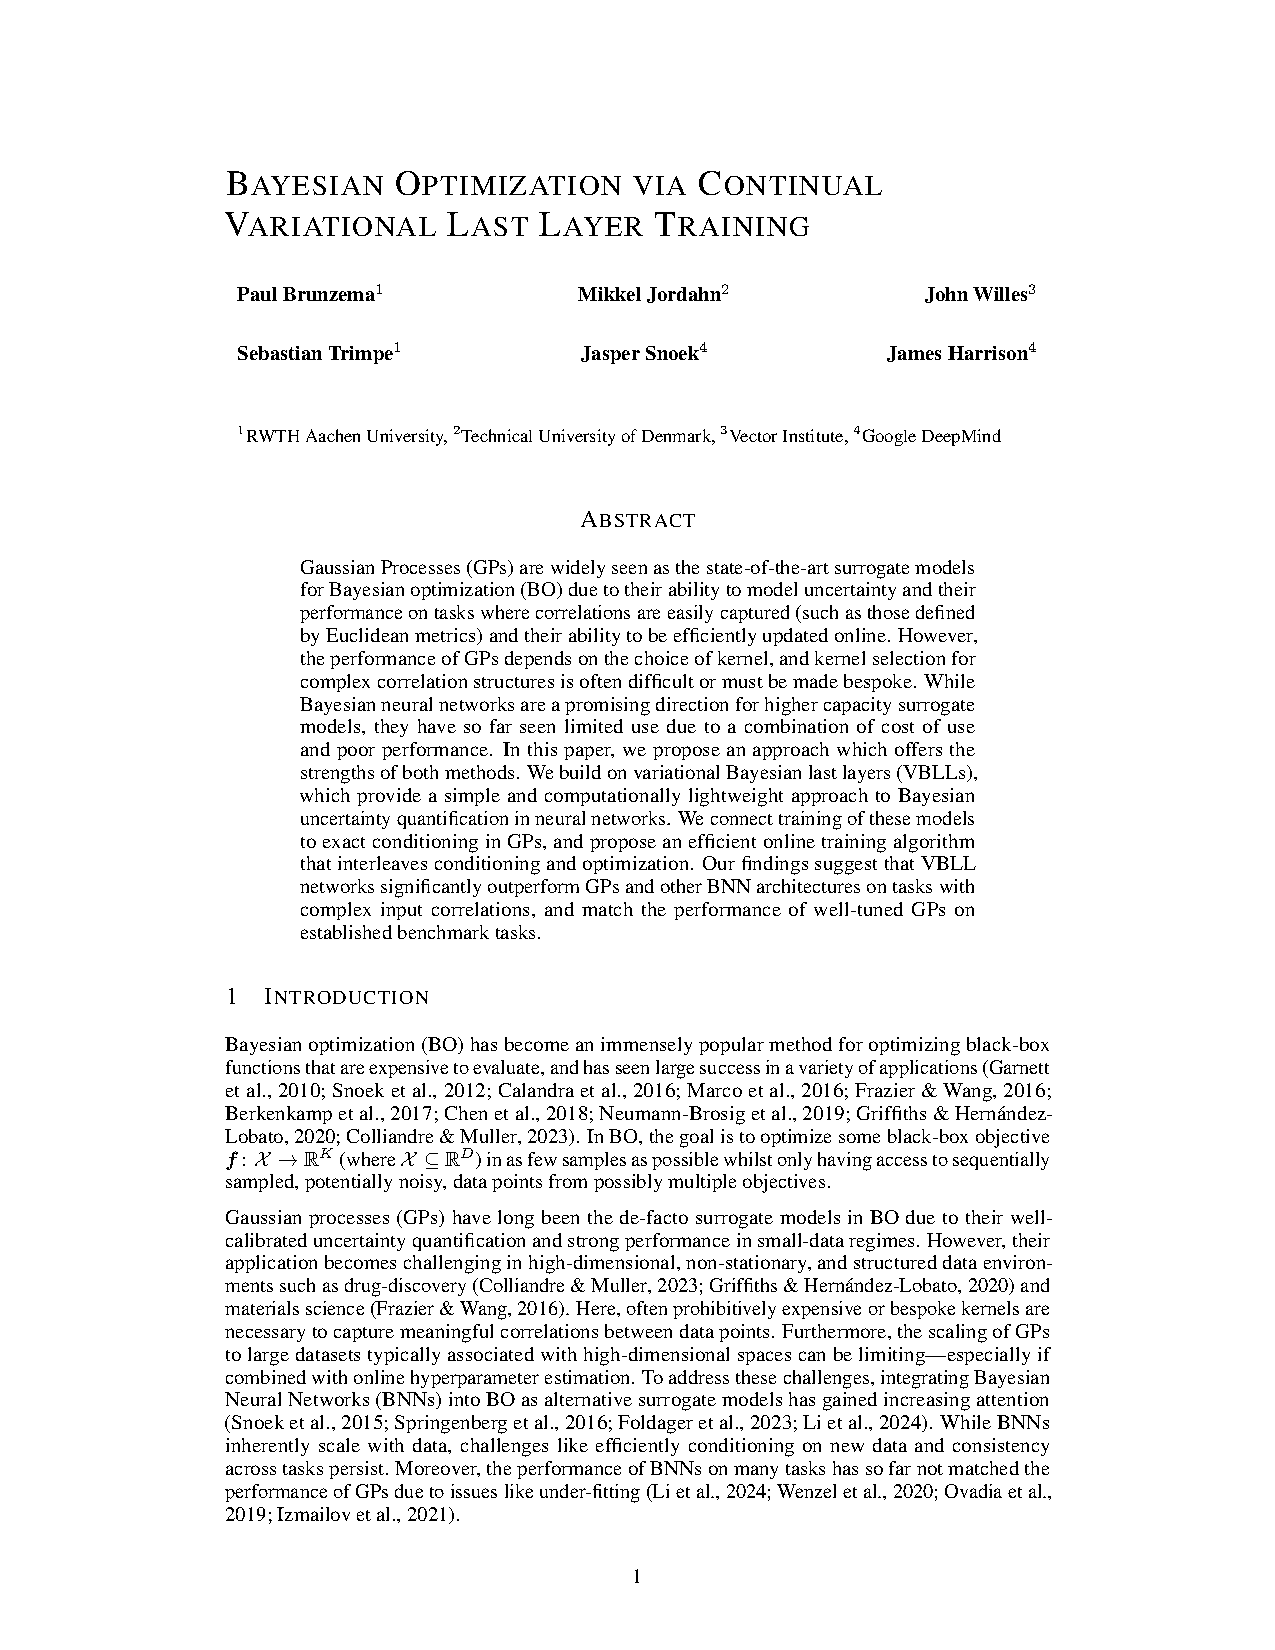
\includepdf[pages=-, offset=0mm 0mm, delta=0mm 0mm, scale=1.0, pagecommand={\thispagestyle{mystuff}{}{}{}}]{chapters/PaperD_VBLLBO/PaperD_ICLR.pdf}